        \begin{definicija}
            \textbf{Trikotnik} je lik/množica točk v ravnini, omejena s tremi daljicami -- \textbf{stranicami} ($a, b, c$), ki povezujejo tri nekolinearne točke ($A, B, C$) v ravnini. Te točke imenujemo \textbf{oglišča} trikotnika.
    
                \begin{figure}[H]
                    \centering
                    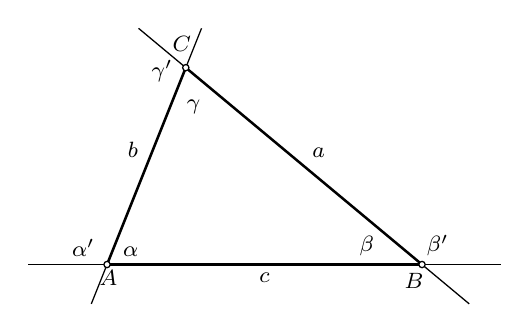
\begin{tikzpicture}
                        % \clip (0,0) rectangle (14.000000,10.000000);
                        {\footnotesize
                        
                        % Marking point A by circle
                        \draw<2-> [line width=0.016cm] (2.000000,1.500000) circle (0.040000);%
                        \draw<2-> (1.800000,1.530000) node [anchor=north west] { $A$ };%
                        
                        % Marking point B by circle
                        \draw<2-> [line width=0.016cm] (6.000000,1.500000) circle (0.040000);%
                        \draw<2-> (5.900000,1.500000) node [anchor=north] { $B$ };%
                        
                        % Marking point C by circle
                        \draw<2-> [line width=0.016cm] (3.000000,4.000000) circle (0.040000);%
                        \draw<2-> (2.950000,4.100000) node [anchor=south] { $C$ };%
                        
                        % Drawing line A B
                        \draw<4-> [line width=0.016cm] (1.000000,1.500000) -- (1.960000,1.500000);%
                        \draw<4-> [line width=0.016cm] (2.040000,1.500000) -- (5.960000,1.500000);%
                        \draw<4-> [line width=0.016cm] (6.040000,1.500000) -- (7.000000,1.500000);%
                        
                        % Drawing line B C
                        \draw<4-> [line width=0.016cm] (6.600000,1.000000) -- (6.030729,1.474393);%
                        \draw<4-> [line width=0.016cm] (5.969271,1.525607) -- (3.030729,3.974393);%
                        \draw<4-> [line width=0.016cm] (2.969271,4.025607) -- (2.400000,4.500000);%
                        
                        % Drawing line A C
                        \draw<4-> [line width=0.016cm] (1.800000,1.000000) -- (1.985144,1.462861);%
                        \draw<4-> [line width=0.016cm] (2.014856,1.537139) -- (2.985144,3.962861);%
                        \draw<4-> [line width=0.016cm] (3.014856,4.037139) -- (3.200000,4.500000);%
                        
                        % Marking point c
                        \draw<2-> (4.000000,1.500000) node [anchor=north] { $c$ };%
                        
                        % Marking point a
                        \draw<2-> (4.500000,2.750000) node [anchor=south west] { $a$ };%
                        
                        % Marking point b
                        \draw<2-> (2.500000,2.750000) node [anchor=south east] { $b$ };%
                        
                        % Marking point \gamma
                        \draw<3-> (3.100000,3.700000) node [anchor=north] { $\gamma$ };%
                        
                        % Marking point \gamma'
                        \draw<4-> (2.700000,4.200000) node [anchor=north] { $\gamma'$ };%
                        
                        % Marking point \beta
                        \draw<3-> (5.300000,1.500000) node [anchor=south] { $\beta$ };%
                        
                        % Marking point \beta'
                        \draw<4-> (6.200000,1.500000) node [anchor=south] { $\beta'$ };%
                        
                        % Marking point \alpha
                        \draw<3-> (2.300000,1.500000) node [anchor=south] { $\alpha$ };%
                        
                        % Marking point \alpha'
                        \draw<4-> (1.700000,1.500000) node [anchor=south] { $\alpha'$ };%
                        
                        % Drawing segment A B
                        \draw<2-> [line width=0.032cm] (2.040000,1.500000) -- (5.960000,1.500000);%
                        
                        % Drawing segment B C
                        \draw<2-> [line width=0.032cm] (5.969271,1.525607) -- (3.030729,3.974393);%
                        
                        % Drawing segment A C
                        \draw<2-> [line width=0.032cm] (2.014856,1.537139) -- (2.985144,3.962861);%
                        }
                    \end{tikzpicture}
                \end{figure}

        \end{definicija}
           

        V trikotniku $\triangle ABC$  so $\alpha, \beta$ in $\gamma$ \textbf{notranji koti}, njihovi sokoti $\alpha', \beta'$ in $\gamma'$ pa so \textbf{zunanji koti}. 
            
        
            
        \begin{izrek}
            Vsota notranjih kotov trikotnika je $180^\circ$: 
            $$\alpha+\beta+\gamma=180^\circ.$$ 
        \end{izrek}

        
        \begin{izrek}
            Zunanji kot trikotnika je enak vsoti notranjih nepriležnih kotov: 

            \begin{align*}
                \alpha' &= \beta+\gamma \\
                \beta' &= \alpha+\gamma \\
                \gamma' &= \alpha+\beta
            \end{align*}
        \end{izrek}

        
        \begin{izrek}
            Vsota zunanjih kotov trikotnika je $360^\circ$: 

            $$\alpha'+\beta'+\gamma'=360^\circ.$$ 
        \end{izrek}




    
        
        \begin{izrek}
            Nasproti daljše stranice trikotnika leži večji notranji kot, nasproti krajše stranice pa manjši notranji kot trikotnika.

            $$a>b \Leftrightarrow \alpha > \beta$$
        \end{izrek}

        
        \begin{Izrek}[Trikotniška neenakost]
            Vsaka stranica trikotnika je krajša od vsote dolžin drugih dveh stranic.

            \begin{align*}
                a &< b + c \\
                b &< a + c \\
                c &< a + b
            \end{align*}
        \end{izrek}

        
        \begin{izrek}
            Vsaka stranica trikotnika je daljša od absolutne vrednosti razlike dolžin drugih dveh stranic.
        \end{izrek}





    

        \begin{definicija}
            \textbf{Višina} na stranico trikotnika je daljica, ki povezuje nosilko te stranice z nasprotnim ogliščem in je pravokotna na to nosilko. 
            Njena dolžina je razdalja oglišča od nasprotne stranice.

        
        \begin{figure}[H]
            \centering
            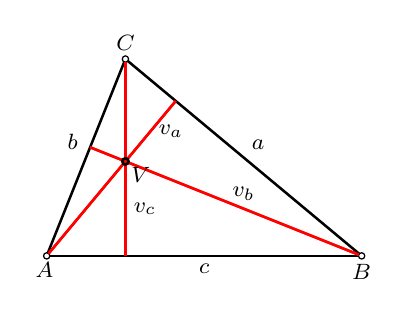
\begin{tikzpicture}
                % \clip (0,0) rectangle (14.000000,10.000000);
                {\footnotesize
                
                % Marking point A by circle
                \draw<1-> [line width=0.016cm] (2.000000,1.500000) circle (0.040000);%
                \draw<1-> (1.970000,1.530000) node [anchor=north] { $A$ };%
                
                % Marking point B by circle
                \draw<1-> [line width=0.016cm] (6.000000,1.500000) circle (0.040000);%
                \draw<1-> (6.000000,1.500000) node [anchor=north] { $B$ };%
                
                % Marking point C by circle
                \draw<1-> [line width=0.016cm] (3.000000,4.000000) circle (0.040000);%
                \draw<1-> (3.000000,4.000000) node [anchor=south] { $C$ };%
                
                % Marking point c
                \draw<1-> (4.000000,1.500000) node [anchor=north] { $c$ };%
                
                % Marking point a
                \draw<1-> (4.500000,2.750000) node [anchor=south west] { $a$ };%
                
                % Marking point b
                \draw<1-> (2.500000,2.750000) node [anchor=south east] { $b$ };%
                
                % Marking point v_a
                \draw<2-> (3.319672,3.083607) node [anchor=west] { $v_a$ };%
                
                % Marking point v_c
                \draw<2-> (3.000000,2.100000) node [anchor=west] { $v_c$ };%
                
                % Marking point v_b
                \draw<2-> (4.500000,2.100000) node [anchor=south] { $v_b$ };%
                
                % Drawing segment A B
                \draw<1-> [line width=0.032cm] (2.040000,1.500000) -- (5.960000,1.500000);%
                
                % Drawing segment B C
                \draw<1-> [line width=0.032cm] (5.969271,1.525607) -- (3.030729,3.974393);%
                
                % Drawing segment A C
                \draw<1-> [line width=0.032cm] (2.014856,1.537139) -- (2.985144,3.962861);%
                
                % Changing color 255 0 0
                \definecolor{r255g0b0}{rgb}{1.000000,0.000000,0.000000}%
                \color{r255g0b0}% 
                
                % Drawing segment A A'
                \draw<2> [line width=0.032cm] (2.025607,1.530729) -- (3.639344,3.467213);%
                \draw<3-> [line width=0.032cm] (2.025607,1.530729) -- (2.974393,2.669271);%
                \draw<3-> [line width=0.032cm] (3.025607,2.730729) -- (3.639344,3.467213);%
                
                % Drawing segment B B'
                \draw<2> [line width=0.032cm] (5.962861,1.514856) -- (2.551724,2.879310);%
                \draw<3-> [line width=0.032cm] (5.962861,1.514856) -- (3.037139,2.685144);%
                \draw<3-> [line width=0.032cm] (2.962861,2.714856) -- (2.551724,2.879310);%
                
                % Drawing segment C C'
                \draw<2> [line width=0.032cm] (3.000000,3.960000) -- (3.000000,1.500000);%
                \draw<3-> [line width=0.032cm] (3.000000,3.960000) -- (3.000000,2.740000);%
                \draw<3-> [line width=0.032cm] (3.000000,2.660000) -- (3.000000,1.500000);%
                
                % Changing color 0 0 0
                \definecolor{r0g0b0}{rgb}{0.000000,0.000000,0.000000}%
                \color{r0g0b0}% 
                
                % Marking point V by circle
                \draw<3-> [line width=0.032cm] (3.000000,2.700000) circle (0.040000);%
                \draw<3-> (2.970000,2.730000) node [anchor=north west] { $V$ };%
                \color{black}
                }
            \end{tikzpicture}
                
        \end{figure}


        \end{definicija}

        \begin{izrek}
            Nosilke vseh treh višin na stranice trikotnika se sekajo v eni točki, ki jo imenujemo \textbf{višinska točka} ali \textbf{ortocenter}.
        \end{izrek}
        


    

        \begin{definicija}
            \textbf{Težiščnica} na stranico trikotnika je daljica, ki povezuje razpolovišče te stranice z nasprotnim ogliščem. 


        \begin{figure}[H]
            \centering
            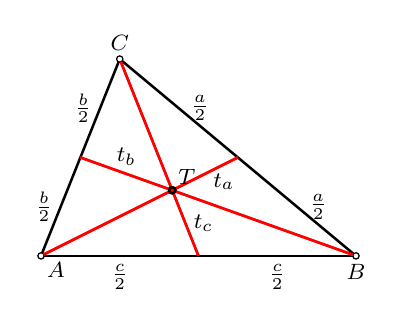
\begin{tikzpicture}
                % \clip (0,0) rectangle (14.000000,10.000000);
                {\footnotesize
                
                % Marking point A by circle
                \draw [line width=0.016cm] (2.000000,1.500000) circle (0.040000);%
                \draw (1.970000,1.530000) node [anchor=north west] { $A$ };%
                
                % Marking point B by circle
                \draw [line width=0.016cm] (6.000000,1.500000) circle (0.040000);%
                \draw (6.000000,1.500000) node [anchor=north] { $B$ };%
                
                % Marking point C by circle
                \draw [line width=0.016cm] (3.000000,4.000000) circle (0.040000);%
                \draw (3.000000,4.000000) node [anchor=south] { $C$ };%
                
                % Marking point t_a
                \draw<2-> (4.083333,2.441667) node [anchor=west] { $t_a$ };%
                
                % Marking point t_c
                \draw<2-> (3.833333,1.916667) node [anchor=west] { $t_c$ };%
                
                % Marking point t_b
                \draw<2-> (3.083333,2.541667) node [anchor=south] { $t_b$ };%
                
                % Marking point \frac{b}{2}
                \draw<2-> (2.250000,2.125000) node [anchor=east] { $\frac{b}{2}$ };%
                
                % Marking point \frac{b}{2}
                \draw<2-> (2.750000,3.375000) node [anchor=east] { $\frac{b}{2}$ };%
                
                % Marking point \frac{c}{2}
                \draw<2-> (3.000000,1.500000) node [anchor=north] { $\frac{c}{2}$ };%
                
                % Marking point \frac{c}{2}
                \draw<2-> (5.000000,1.500000) node [anchor=north] { $\frac{c}{2}$ };%
                
                % Marking point \frac{a}{2}
                \draw<2-> (5.30000,2.125000) node [anchor=west] { $\frac{a}{2}$ };%
                
                % Marking point \frac{a}{2}
                \draw<2-> (3.80000,3.375000) node [anchor=west] { $\frac{a}{2}$ };%
                
                % Drawing segment A B
                \draw [line width=0.032cm] (2.040000,1.500000) -- (5.960000,1.500000);%
                
                % Drawing segment B C
                \draw [line width=0.032cm] (5.969271,1.525607) -- (3.030729,3.974393);%
                
                % Drawing segment A C
                \draw [line width=0.032cm] (2.014856,1.537139) -- (2.985144,3.962861);%
                
                % Changing color 255 0 0
                \definecolor{r255g0b0}{rgb}{1.000000,0.000000,0.000000}%
                \color{r255g0b0}% 
                
                % Drawing segment A a
                \draw<2> [line width=0.032cm] (2.035777,1.517889) -- (4.500000,2.750000);%
                \draw<3-> [line width=0.032cm] (2.035777,1.517889) -- (3.630890,2.315445);%
                \draw<3-> [line width=0.032cm] (3.702444,2.351222) -- (4.500000,2.750000);%
                
                % Drawing segment B b
                \draw<2> [line width=0.032cm] (5.962330,1.513453) -- (2.500000,2.750000);%
                \draw<3-> [line width=0.032cm] (5.962330,1.513453) -- (3.704336,2.319880);%
                \draw<3-> [line width=0.032cm] (3.628997,2.346787) -- (2.500000,2.750000);%
                
                % Drawing segment C c
                \draw<2> [line width=0.032cm] (3.014856,3.962861) -- (4.000000,1.500000);%
                \draw<3-> [line width=0.032cm] (3.014856,3.962861) -- (3.651811,2.370472);%
                \draw<3-> [line width=0.032cm] (3.681522,2.296194) -- (4.000000,1.500000);%
                
                % Changing color 0 0 0
                \definecolor{r0g0b0}{rgb}{0.000000,0.000000,0.000000}%
                \color{r0g0b0}% 
                
                % Marking point T by circle
                \draw<3-> [line width=0.032cm] (3.666667,2.333333) circle (0.040000);%
                \draw<3-> (3.636667,2.303333) node [anchor=south west] { $T$ };%
                \color{black}
                }
            \end{tikzpicture}
                
        \end{figure}

        \end{definicija}


        \begin{izrek}
            Vse tri trikotnikove težiščnice se sekajo v eni točki -- \textbf{težišču} ali \textbf{baricentru} trikotnika. \\ 
            Težišče deli težiščnico v razmerju $1:2$.
        \end{izrek}
        

    


    

        \begin{izrek}
            Simetrale vseh treh stranic trikotnika se sekajo v eni točki --  \textbf{središču trikotniku očrtane krožnice}. 


        \begin{figure}[H]
            \centering
            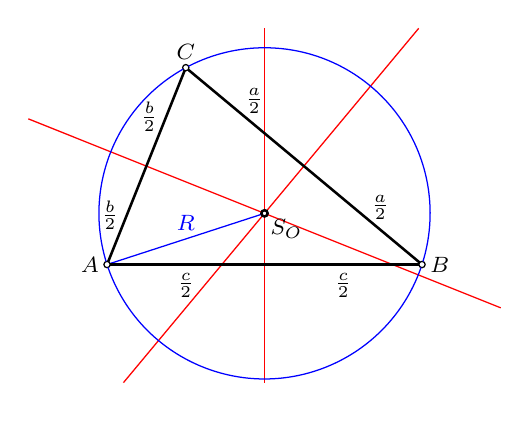
\begin{tikzpicture}
                % \clip (0,0) rectangle (14.000000,10.000000);
                {\footnotesize
                
                % Marking point A by circle
                \draw [line width=0.016cm] (2.000000,2.500000) circle (0.040000);%
                \draw (2.000000,2.500000) node [anchor=east] { $A$ };%
                
                % Marking point B by circle
                \draw [line width=0.016cm] (6.000000,2.500000) circle (0.040000);%
                \draw (6.000000,2.500000) node [anchor=west] { $B$ };%
                
                % Marking point C by circle
                \draw [line width=0.016cm] (3.000000,5.000000) circle (0.040000);%
                \draw (3.000000,5.000000) node [anchor=south] { $C$ };%
                
                % Marking point \frac{b}{2}
                \draw (2.250000,3.125000) node [anchor=east] { $\frac{b}{2}$ };%
                
                % Marking point \frac{b}{2}
                \draw (2.750000,4.375000) node [anchor=east] { $\frac{b}{2}$ };%
                
                % Marking point \frac{c}{2}
                \draw (3.000000,2.500000) node [anchor=north] { $\frac{c}{2}$ };%
                
                % Marking point \frac{c}{2}
                \draw (5.000000,2.500000) node [anchor=north] { $\frac{c}{2}$ };%
                
                % Marking point \frac{a}{2}
                \draw (5.250000,3.225000) node [anchor=west] { $\frac{a}{2}$ };%
                
                % Marking point \frac{a}{2}
                \draw (3.650000,4.575000) node [anchor=west] { $\frac{a}{2}$ };%
                
                % Changing color 255 0 0
                \definecolor{r255g0b0}{rgb}{1.000000,0.000000,0.000000}%
                \color{r255g0b0}% 
                
                % Drawing line s_c
                \draw [line width=0.016cm] (4.000000,1.000000) -- (4.000000,3.110000);%
                \draw [line width=0.016cm] (4.000000,3.190000) -- (4.000000,5.500000);%
                
                % Drawing line s_a
                \draw [line width=0.016cm] (2.208333,1.000000) -- (3.974393,3.119271);%
                \draw [line width=0.016cm] (4.025607,3.180729) -- (5.958333,5.500000);%
                
                % Drawing line s_b
                \draw [line width=0.016cm] (1.000000,4.350000) -- (3.962861,3.164856);%
                \draw [line width=0.016cm] (4.037139,3.135144) -- (7.000000,1.950000);%
                
                % Changing color 0 0 255
                \definecolor{r0g0b255}{rgb}{0.000000,0.000000,1.000000}%
                \color{r0g0b255}% 
                
                % Drawing circle S_O A
                \draw [line width=0.016cm] (2.012724,2.462079) -- (2.023851,2.430741) arc (200:340:2.102974 and 2.102974) -- (5.987275,2.462077);%
                \draw [line width=0.016cm] (6.012001,2.538157) -- (6.021508,2.570341) arc (344:360:2.102974 and 2.102974) --(6.102974,3.150000) arc (0:117:2.102974 and 2.102974) -- (3.035368,5.018685);%
                \draw [line width=0.016cm] (2.964994,4.980646) -- (2.948513,4.971229) arc (120:196:2.102974 and 2.102974) -- (1.987999,2.538158);%
                
                % Drawing segment A S_O
                \draw [line width=0.016cm] (2.038041,2.512363) -- (3.961959,3.137637);%
                
                % Marking point R
                \draw (3.000000,2.825000) node [anchor=south] { $R$ };%
                
                % Changing color 0 0 0
                \definecolor{r0g0b0}{rgb}{0.000000,0.000000,0.000000}%
                \color{r0g0b0}% 
                
                % Drawing segment A B
                \draw [line width=0.032cm] (2.040000,2.500000) -- (5.960000,2.500000);%
                
                % Drawing segment B C
                \draw [line width=0.032cm] (5.969271,2.525607) -- (3.030729,4.974393);%
                
                % Drawing segment A C
                \draw [line width=0.032cm] (2.014856,2.537139) -- (2.985144,4.962861);%
                
                % Marking point S_O by circle
                \draw [line width=0.032cm] (4.000000,3.150000) circle (0.040000);%
                \draw (3.970000,3.180000) node [anchor=north west] { $S_O$ };%
                \color{black}
                }
            \end{tikzpicture}    

        \end{figure}

        \end{izrek}


        
            Očrtana krožnica poteka skozi vsa oglišča trikotnika. Vse stranice trikotnika so tetive krožnice.


    


    

        \begin{izrek}
            Simetrale notranjih kotov trikotnika se sekajo v eni točki. Ta točka je \textbf{središče trikotniku včrtane krožnice}.


        \begin{figure}[H]
            \centering
            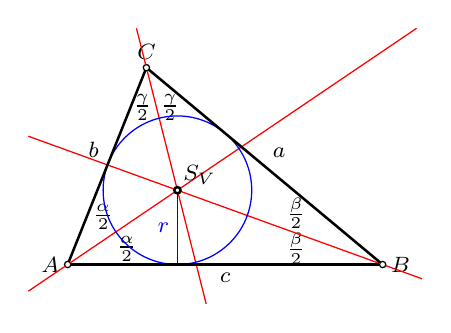
\begin{tikzpicture}
                % \clip (0,0) rectangle (14.000000,10.000000);
                {\footnotesize
                
                % Marking point A by circle
                \draw [line width=0.016cm] (2.000000,2.500000) circle (0.040000);%
                \draw (2.000000,2.500000) node [anchor=east] { $A$ };%
                
                % Marking point B by circle
                \draw [line width=0.016cm] (6.000000,2.500000) circle (0.040000);%
                \draw (6.000000,2.500000) node [anchor=west] { $B$ };%
                
                % Marking point C by circle
                \draw [line width=0.016cm] (3.000000,5.000000) circle (0.040000);%
                \draw (3.000000,5.000000) node [anchor=south] { $C$ };%
                
                % Marking point b
                \draw (2.500000,3.750000) node [anchor=south east] { $b$ };%
                
                % Marking point c
                \draw (4.000000,2.500000) node [anchor=north] { $c$ };%
                
                % Marking point a
                \draw (4.500000,3.750000) node [anchor=south west] { $a$ };%
                
                % Marking point \frac{\alpha}{2}
                \draw (2.750000,2.700000) node  { $\frac{\alpha}{2}$ };%
                
                % Marking point \frac{\gamma}{2}
                \draw (2.950000,4.500000) node  { $\frac{\gamma}{2}$ };%
                
                % Marking point \frac{\alpha}{2}
                \draw (2.450000,3.100000) node  { $\frac{\alpha}{2}$ };%
                
                % Marking point \frac{\beta}{2}
                \draw (4.900000,2.700000) node  { $\frac{\beta}{2}$ };%
                
                % Marking point \frac{\beta}{2}
                \draw (4.900000,3.150000) node  { $\frac{\beta}{2}$ };%
                
                % Marking point \frac{\gamma}{2}
                \draw (3.300000,4.500000) node  { $\frac{\gamma}{2}$ };%
                
                % Changing color 255 0 0
                \definecolor{r255g0b0}{rgb}{1.000000,0.000000,0.000000}%
                \color{r255g0b0}% 
                
                % Drawing line s_c
                \draw [line width=0.016cm] (3.758922,2.000000) -- (3.403539,3.404822);%
                \draw [line width=0.016cm] (3.383919,3.482379) -- (3.009810,4.961222);%
                \draw [line width=0.016cm] (2.990190,5.038778) -- (2.873513,5.500000);%
                
                % Drawing line s_a
                \draw [line width=0.016cm] (6.431099,5.500000) -- (3.426851,3.466025);%
                \draw [line width=0.016cm] (3.360606,3.421175) -- (2.033123,2.522425);%
                \draw [line width=0.016cm] (1.966877,2.477575) -- (1.500000,2.161484);%
                
                % Drawing line s_b
                \draw [line width=0.016cm] (1.500000,4.129225) -- (3.356118,3.457217);%
                \draw [line width=0.016cm] (3.431340,3.429983) -- (5.962389,2.513617);%
                \draw [line width=0.016cm] (6.037611,2.486383) -- (6.500000,2.318975);%
                
                % Changing color 0 0 255
                \definecolor{r0g0b255}{rgb}{0.000000,0.000000,1.000000}%
                \color{r0g0b255}% 
                
                % Drawing circle S_V X
                \draw [line width=0.016cm] (3.393729,3.443600) circle (0.943600);%
                
                % Drawing segment X S_V
                \draw [line width=0.016cm] (3.393729,2.500000) -- (3.393729,3.403600);%
                
                % Marking point r
                \draw (3.393729,2.971800) node [anchor=east] { $r$ };%
                
                % Changing color 0 0 0
                \definecolor{r0g0b0}{rgb}{0.000000,0.000000,0.000000}%
                \color{r0g0b0}% 
                
                % Drawing segment A B
                \draw [line width=0.032cm] (2.040000,2.500000) -- (5.960000,2.500000);%
                
                % Drawing segment B C
                \draw [line width=0.032cm] (5.969271,2.525607) -- (3.030729,4.974393);%
                
                % Drawing segment A C
                \draw [line width=0.032cm] (2.014856,2.537139) -- (2.985144,4.962861);%
                
                % Marking point S_V by circle
                \draw [line width=0.032cm] (3.393729,3.443600) circle (0.040000);%
                \draw (3.363729,3.413600) node [anchor=south west] { $S_V$ };%
                \color{black}
                }
            \end{tikzpicture}
                
        \end{figure}

        \end{izrek}


        
            Včrtana krožnica ima vse tri stranice trikotnika za tangente.



    

        
            Težišče, središče trikotniku očrtane kroznice, središče trikotniku včrtane krožnice in višinska točka so \textbf{znamenite točke trikotnika}.

        
        \begin{izrek}
            Višinska točka, središče očrtane krožnice in težišče so vedno kolinearne. Premico, ki jih povezuje, imenujemo \textbf{Eulerjeva premica}.


            \begin{figure}[H]
                \centering
                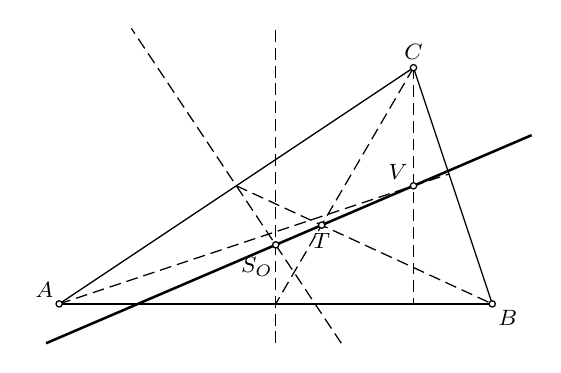
\begin{tikzpicture}
                    % \clip (0,0) rectangle (14.000000,10.000000);
                    {\footnotesize
                    
                    % Drawing segment A B
                    \draw [line width=0.016cm] (1.540000,3.500000) -- (6.960000,3.500000);%
                    
                    % Drawing segment A C
                    \draw [line width=0.016cm] (1.533282,3.522188) -- (5.966718,6.477812);%
                    
                    % Drawing segment B C
                    \draw [line width=0.016cm] (6.987351,3.537947) -- (6.012649,6.462053);%
                    
                    % Drawing line b
                    \draw [line width=0.016cm] (5.083333,3.000000) -- (5.000128,3.124808);%
                    \draw [line width=0.016cm] (4.958526,3.187211) -- (4.875321,3.312019);%
                    \draw [line width=0.016cm] (4.833718,3.374423) -- (4.750513,3.499230);%
                    \draw [line width=0.016cm] (4.708911,3.561634) -- (4.625706,3.686441);%
                    \draw [line width=0.016cm] (4.584103,3.748845) -- (4.500898,3.873653);%
                    \draw [line width=0.016cm] (4.459296,3.936057) -- (4.376091,4.060864);%
                    \draw [line width=0.016cm] (4.334488,4.123268) -- (4.272188,4.216718);%
                    \draw [line width=0.016cm] (4.209681,4.310479) -- (4.126475,4.435287);%
                    \draw [line width=0.016cm] (4.084873,4.497691) -- (4.001668,4.622498);%
                    \draw [line width=0.016cm] (3.960065,4.684902) -- (3.876860,4.809709);%
                    \draw [line width=0.016cm] (3.835258,4.872113) -- (3.752053,4.996921);%
                    \draw [line width=0.016cm] (3.710450,5.059324) -- (3.627245,5.184132);%
                    \draw [line width=0.016cm] (3.585643,5.246536) -- (3.502438,5.371343);%
                    \draw [line width=0.016cm] (3.460835,5.433747) -- (3.377630,5.558555);%
                    \draw [line width=0.016cm] (3.336028,5.620958) -- (3.252823,5.745766);%
                    \draw [line width=0.016cm] (3.211220,5.808170) -- (3.128015,5.932977);%
                    \draw [line width=0.016cm] (3.086413,5.995381) -- (3.003208,6.120189);%
                    \draw [line width=0.016cm] (2.961605,6.182592) -- (2.878400,6.307400);%
                    \draw [line width=0.016cm] (2.836798,6.369804) -- (2.753593,6.494611);%
                    \draw [line width=0.016cm] (2.711990,6.557015) -- (2.628785,6.681823);%
                    \draw [line width=0.016cm] (2.587182,6.744226) -- (2.503977,6.869034);%
                    \draw [line width=0.016cm] (2.462375,6.931438) -- (2.416667,7.000000);%
                    
                    % Drawing line c
                    \draw [line width=0.016cm] (4.250000,3.000000) -- (4.250000,3.150000);%
                    \draw [line width=0.016cm] (4.250000,3.225000) -- (4.250000,3.375000);%
                    \draw [line width=0.016cm] (4.250000,3.450000) -- (4.250000,3.600000);%
                    \draw [line width=0.016cm] (4.250000,3.675000) -- (4.250000,3.825000);%
                    \draw [line width=0.016cm] (4.250000,3.900000) -- (4.250000,4.050000);%
                    \draw [line width=0.016cm] (4.250000,4.125000) -- (4.250000,4.210000);%
                    \draw [line width=0.016cm] (4.250000,4.350000) -- (4.250000,4.500000);%
                    \draw [line width=0.016cm] (4.250000,4.575000) -- (4.250000,4.725000);%
                    \draw [line width=0.016cm] (4.250000,4.800000) -- (4.250000,4.950000);%
                    \draw [line width=0.016cm] (4.250000,5.025000) -- (4.250000,5.175000);%
                    \draw [line width=0.016cm] (4.250000,5.250000) -- (4.250000,5.400000);%
                    \draw [line width=0.016cm] (4.250000,5.475000) -- (4.250000,5.625000);%
                    \draw [line width=0.016cm] (4.250000,5.700000) -- (4.250000,5.850000);%
                    \draw [line width=0.016cm] (4.250000,5.925000) -- (4.250000,6.075000);%
                    \draw [line width=0.016cm] (4.250000,6.150000) -- (4.250000,6.300000);%
                    \draw [line width=0.016cm] (4.250000,6.375000) -- (4.250000,6.525000);%
                    \draw [line width=0.016cm] (4.250000,6.600000) -- (4.250000,6.750000);%
                    \draw [line width=0.016cm] (4.250000,6.825000) -- (4.250000,6.975000);%
                    
                    % Drawing segment C C'
                    \draw [line width=0.016cm] (5.979845,6.465449) -- (5.924419,6.370433);%
                    \draw [line width=0.016cm] (5.886629,6.305650) -- (5.811048,6.176083);%
                    \draw [line width=0.016cm] (5.773258,6.111299) -- (5.697677,5.981733);%
                    \draw [line width=0.016cm] (5.659887,5.916949) -- (5.584306,5.787382);%
                    \draw [line width=0.016cm] (5.546516,5.722599) -- (5.470935,5.593032);%
                    \draw [line width=0.016cm] (5.433145,5.528249) -- (5.357564,5.398682);%
                    \draw [line width=0.016cm] (5.319774,5.333898) -- (5.244193,5.204332);%
                    \draw [line width=0.016cm] (5.206403,5.139548) -- (5.130822,5.009981);%
                    \draw [line width=0.016cm] (5.093032,4.945198) -- (5.017452,4.815631);%
                    \draw [line width=0.016cm] (4.979661,4.750848) -- (4.904081,4.621281);%
                    \draw [line width=0.016cm] (4.866290,4.556497) -- (4.853488,4.534551);%
                    \draw [line width=0.016cm] (4.813178,4.465449) -- (4.790710,4.426931);%
                    \draw [line width=0.016cm] (4.752919,4.362147) -- (4.677339,4.232580);%
                    \draw [line width=0.016cm] (4.639548,4.167797) -- (4.563968,4.038230);%
                    \draw [line width=0.016cm] (4.526177,3.973447) -- (4.450597,3.843880);%
                    \draw [line width=0.016cm] (4.412806,3.779096) -- (4.337226,3.649530);%
                    \draw [line width=0.016cm] (4.299435,3.584746) -- (4.250000,3.500000);%
                    
                    % Drawing segment C U
                    \draw [line width=0.016cm] (6.000000,6.460000) -- (6.000000,6.350000);%
                    \draw [line width=0.016cm] (6.000000,6.275000) -- (6.000000,6.125000);%
                    \draw [line width=0.016cm] (6.000000,6.050000) -- (6.000000,5.900000);%
                    \draw [line width=0.016cm] (6.000000,5.825000) -- (6.000000,5.675000);%
                    \draw [line width=0.016cm] (6.000000,5.600000) -- (6.000000,5.450000);%
                    \draw [line width=0.016cm] (6.000000,5.375000) -- (6.000000,5.225000);%
                    \draw [line width=0.016cm] (6.000000,5.150000) -- (6.000000,5.040000);%
                    \draw [line width=0.016cm] (6.000000,4.925000) -- (6.000000,4.775000);%
                    \draw [line width=0.016cm] (6.000000,4.700000) -- (6.000000,4.550000);%
                    \draw [line width=0.016cm] (6.000000,4.475000) -- (6.000000,4.325000);%
                    \draw [line width=0.016cm] (6.000000,4.250000) -- (6.000000,4.100000);%
                    \draw [line width=0.016cm] (6.000000,4.025000) -- (6.000000,3.875000);%
                    \draw [line width=0.016cm] (6.000000,3.800000) -- (6.000000,3.650000);%
                    \draw [line width=0.016cm] (6.000000,3.575000) -- (6.000000,3.500000);%
                    
                    % Drawing segment A V
                    \draw [line width=0.016cm] (1.537947,3.512649) -- (1.642302,3.547434);%
                    \draw [line width=0.016cm] (1.713454,3.571151) -- (1.855756,3.618585);%
                    \draw [line width=0.016cm] (1.926907,3.642302) -- (2.069210,3.689737);%
                    \draw [line width=0.016cm] (2.140361,3.713454) -- (2.282664,3.760888);%
                    \draw [line width=0.016cm] (2.353815,3.784605) -- (2.496117,3.832039);%
                    \draw [line width=0.016cm] (2.567269,3.855756) -- (2.709571,3.903190);%
                    \draw [line width=0.016cm] (2.780722,3.926907) -- (2.923025,3.974342);%
                    \draw [line width=0.016cm] (2.994176,3.998059) -- (3.136479,4.045493);%
                    \draw [line width=0.016cm] (3.207630,4.069210) -- (3.349932,4.116644);%
                    \draw [line width=0.016cm] (3.421084,4.140361) -- (3.563386,4.187795);%
                    \draw [line width=0.016cm] (3.634537,4.211512) -- (3.776840,4.258947);%
                    \draw [line width=0.016cm] (3.847991,4.282664) -- (3.990294,4.330098);%
                    \draw [line width=0.016cm] (4.061445,4.353815) -- (4.203747,4.401249);%
                    \draw [line width=0.016cm] (4.274899,4.424966) -- (4.417201,4.472400);%
                    \draw [line width=0.016cm] (4.488352,4.496117) -- (4.630655,4.543552);%
                    \draw [line width=0.016cm] (4.701806,4.567269) -- (4.844109,4.614703);%
                    \draw [line width=0.016cm] (4.915260,4.638420) -- (5.057562,4.685854);%
                    \draw [line width=0.016cm] (5.128714,4.709571) -- (5.271016,4.757005);%
                    \draw [line width=0.016cm] (5.342167,4.780722) -- (5.484470,4.828157);%
                    \draw [line width=0.016cm] (5.555621,4.851874) -- (5.697924,4.899308);%
                    \draw [line width=0.016cm] (5.769075,4.923025) -- (5.911377,4.970459);%
                    \draw [line width=0.016cm] (6.037947,5.012649) -- (6.124831,5.041610);%
                    \draw [line width=0.016cm] (6.195982,5.065327) -- (6.338285,5.112762);%
                    \draw [line width=0.016cm] (6.409436,5.136479) -- (6.450000,5.150000);%
                    
                    % Drawing segment B' B
                    \draw [line width=0.016cm] (3.750000,5.000000) -- (3.886194,4.937141);%
                    \draw [line width=0.016cm] (3.954291,4.905712) -- (4.090485,4.842853);%
                    \draw [line width=0.016cm] (4.158582,4.811424) -- (4.294776,4.748565);%
                    \draw [line width=0.016cm] (4.362873,4.717136) -- (4.499066,4.654277);%
                    \draw [line width=0.016cm] (4.567163,4.622848) -- (4.703357,4.559989);%
                    \draw [line width=0.016cm] (4.771454,4.528560) -- (4.797015,4.516762);%
                    \draw [line width=0.016cm] (4.869652,4.483238) -- (4.907648,4.465701);%
                    \draw [line width=0.016cm] (4.975745,4.434271) -- (5.111939,4.371413);%
                    \draw [line width=0.016cm] (5.180036,4.339983) -- (5.316230,4.277125);%
                    \draw [line width=0.016cm] (5.384327,4.245695) -- (5.520521,4.182837);%
                    \draw [line width=0.016cm] (5.588618,4.151407) -- (5.724812,4.088548);%
                    \draw [line width=0.016cm] (5.792909,4.057119) -- (5.929103,3.994260);%
                    \draw [line width=0.016cm] (5.997199,3.962831) -- (6.133393,3.899972);%
                    \draw [line width=0.016cm] (6.201490,3.868543) -- (6.337684,3.805684);%
                    \draw [line width=0.016cm] (6.405781,3.774255) -- (6.541975,3.711396);%
                    \draw [line width=0.016cm] (6.610072,3.679967) -- (6.746266,3.617108);%
                    \draw [line width=0.016cm] (6.814363,3.585679) -- (6.950557,3.522820);%
                    
                    % Marking point A by circle
                    \draw [line width=0.016cm] (1.500000,3.500000) circle (0.040000);%
                    \draw (1.530000,3.470000) node [anchor=south east] { $A$ };%
                    
                    % Marking point B by circle
                    \draw [line width=0.016cm] (7.000000,3.500000) circle (0.040000);%
                    \draw (6.970000,3.530000) node [anchor=north west] { $B$ };%
                    
                    % Marking point C by circle
                    \draw [line width=0.016cm] (6.000000,6.500000) circle (0.040000);%
                    \draw (6.000000,6.500000) node [anchor=south] { $C$ };%
                    
                    % Marking point O by circle
                    \draw [line width=0.016cm] (4.250000,4.250000) circle (0.040000);%
                    \draw (4.320000,4.200000) node [anchor=north east] { $S_O$ };%
                    
                    % Marking point T by circle
                    \draw [line width=0.016cm] (4.833333,4.500000) circle (0.040000);%
                    \draw (4.833333,4.500000) node [anchor=north] { $T$ };%
                    
                    % Marking point H_C by circle
                    \draw [line width=0.016cm] (6.000000,5.000000) circle (0.040000);%
                    \draw (6.030000,4.970000) node [anchor=south east] { $V$ };%
                    
                    % Drawing line O T
                    \draw [line width=0.032cm] (1.333333,3.000000) -- (4.213234,4.234243);%
                    \draw [line width=0.032cm] (4.286766,4.265757) -- (4.796568,4.484243);%
                    \draw [line width=0.032cm] (4.870099,4.515757) -- (5.963234,4.984243);%
                    \draw [line width=0.032cm] (6.036766,5.015757) -- (7.500000,5.642857);%
                    }
                \end{tikzpicture}
                    
            \end{figure}

        \end{izrek}

    





    
        \subsubsection*{Vrste trikotnikov glede na stranice}

        RAZNOSTRANIČNI TRIKOTNIK 

                \begin{figure}[H]
                    \centering
                    \begin{tikzpicture}
                        % \clip (0,0) rectangle (14.000000,10.000000);
                        {\footnotesize
                        
                        % Marking point A by circle
                        \draw [line width=0.016cm] (1.500000,1.500000) circle (0.040000);%
                        \draw (1.500000,1.500000) node [anchor=north] { $A$ };%
                        
                        % Marking point B by circle
                        \draw [line width=0.016cm] (6.000000,1.500000) circle (0.040000);%
                        \draw (6.000000,1.500000) node [anchor=north] { $B$ };%
                        
                        % Marking point C by circle
                        \draw [line width=0.016cm] (4.500000,4.500000) circle (0.040000);%
                        \draw (4.500000,4.500000) node [anchor=south] { $C$ };%
                        
                        % Changing color 255 0 0
                        \definecolor{r255g0b0}{rgb}{1.000000,0.000000,0.000000}%
                        \color{r255g0b0}% 
                        
                        % Drawing segment B C
                        \draw [line width=0.016cm] (5.982111,1.535777) -- (4.517889,4.464223);%
                        
                        % Marking point a
                        \draw (5.250000,3.000000) node [anchor=south west] { $a$ };%
                        
                        % Changing color 0 255 0
                        \definecolor{r0g255b0}{rgb}{0.000000,1.000000,0.000000}%
                        \color{r0g255b0}% 
                        
                        % Drawing segment A C
                        \draw [line width=0.016cm] (1.528284,1.528284) -- (4.471716,4.471716);%
                        
                        % Marking point b
                        \draw (3.000000,3.000000) node [anchor=south east] { $b$ };%
                        
                        % Changing color 0 0 255
                        \definecolor{r0g0b255}{rgb}{0.000000,0.000000,1.000000}%
                        \color{r0g0b255}% 
                        
                        % Drawing segment A B
                        \draw [line width=0.016cm] (1.540000,1.500000) -- (5.960000,1.500000);%
                        
                        % Marking point c
                        \draw (3.750000,1.500000) node [anchor=north] { $c$ };%
                        \color{black}
                        }
                    \end{tikzpicture}
                        
                \end{figure}

                vse tri stranice različno dolge 
                % $\Rightarrow$ vsi trije koti so različni
                

                ENAKOKRAKI TRIKOTNIK 

                \begin{figure}[H]
                    \centering
                    \begin{tikzpicture}
                        % \clip (0,0) rectangle (14.000000,10.000000);
                        {\footnotesize
                        
                        % Marking point A by circle
                        \draw [line width=0.016cm] (1.500000,1.500000) circle (0.040000);%
                        \draw (1.500000,1.500000) node [anchor=north] { $A$ };%
                        
                        % Marking point B by circle
                        \draw [line width=0.016cm] (5.000000,1.500000) circle (0.040000);%
                        \draw (5.000000,1.500000) node [anchor=north] { $B$ };%
                        
                        % Marking point C by circle
                        \draw [line width=0.016cm] (3.250000,5.000000) circle (0.040000);%
                        \draw (3.250000,5.000000) node [anchor=south] { $C$ };%
                        
                        % Changing color 255 0 0
                        \definecolor{r255g0b0}{rgb}{1.000000,0.000000,0.000000}%
                        \color{r255g0b0}% 
                        
                        % Drawing segment B C
                        \draw [line width=0.016cm] (4.982111,1.535777) -- (3.267889,4.964223);%
                        
                        % Marking point a
                        \draw (4.125000,3.250000) node [anchor=south west] { $a$ };%
                        
                        % Drawing segment A C
                        \draw [line width=0.016cm] (1.517889,1.535777) -- (3.232111,4.964223);%
                        
                        % Marking point a
                        \draw (2.375000,3.250000) node [anchor=south east] { $a$ };%
                        
                        % Changing color 0 0 255
                        \definecolor{r0g0b255}{rgb}{0.000000,0.000000,1.000000}%
                        \color{r0g0b255}% 
                        
                        % Drawing segment A B
                        \draw [line width=0.016cm] (1.540000,1.500000) -- (4.960000,1.500000);%
                        
                        % Marking point c
                        \draw (3.250000,1.500000) node [anchor=north] { $c$ };%
                        \color{black}
                        }
                    \end{tikzpicture}
                        
                \end{figure}

                dve stranici enako dolgi 
                % $\Rightarrow$ kota ob osnovnici sta skladna
                


                ENAKOSTRANIČNI ali PRAVILNI TRIKOTNIK 

                \begin{figure}[H]
                    \centering
                    \begin{tikzpicture}
                        % \clip (0,0) rectangle (14.000000,10.000000);
                        {\footnotesize
                        
                        % Marking point A by circle
                        \draw [line width=0.016cm] (1.500000,1.500000) circle (0.040000);%
                        \draw (1.500000,1.500000) node [anchor=north] { $A$ };%
                        
                        % Marking point B by circle
                        \draw [line width=0.016cm] (5.500000,1.500000) circle (0.040000);%
                        \draw (5.500000,1.500000) node [anchor=north] { $B$ };%
                        
                        % Marking point C by circle
                        \draw [line width=0.016cm] (3.500000,5.000000) circle (0.040000);%
                        \draw (3.500000,5.000000) node [anchor=south] { $C$ };%
                        
                        % Changing color 0 255 0
                        \definecolor{r0g255b0}{rgb}{0.000000,1.000000,0.000000}%
                        \color{r0g255b0}% 
                        
                        % Drawing segment B C
                        \draw [line width=0.016cm] (5.480154,1.534730) -- (3.519846,4.965270);%
                        
                        % Marking point a
                        \draw (4.500000,3.250000) node [anchor=south west] { $a$ };%
                        
                        % Drawing segment A C
                        \draw [line width=0.016cm] (1.519846,1.534730) -- (3.480154,4.965270);%
                        
                        % Marking point a
                        \draw (2.500000,3.250000) node [anchor=south east] { $a$ };%
                        
                        % Drawing segment A B
                        \draw [line width=0.016cm] (1.540000,1.500000) -- (5.460000,1.500000);%
                        
                        % Marking point a
                        \draw (3.500000,1.500000) node [anchor=north] { $a$ };%
                        \color{black}
                        }
                    \end{tikzpicture}
                        
                \end{figure}

                vse tri stranice enako dolge 
                % $\Rightarrow$ vsi trije koti so skladni
                


    

    
        \subsubsection*{Vrste trikotnikov glede na kote}


        OSTROKOTNI TRIKOTNIK 

                \begin{figure}[H]
                    \centering
                    \begin{tikzpicture}
                        % \clip (0,0) rectangle (14.000000,10.000000);
                        {\footnotesize
                        
                        % Marking point A by circle
                        \draw [line width=0.016cm] (1.500000,1.500000) circle (0.040000);%
                        \draw (1.500000,1.500000) node [anchor=north] { $A$ };%
                        
                        % Marking point B by circle
                        \draw [line width=0.016cm] (6.000000,1.500000) circle (0.040000);%
                        \draw (6.000000,1.500000) node [anchor=north] { $B$ };%
                        
                        % Marking point C by circle
                        \draw [line width=0.016cm] (4.500000,4.500000) circle (0.040000);%
                        \draw (4.500000,4.500000) node [anchor=south] { $C$ };%
                        
                        % Drawing segment A B
                        \draw [line width=0.016cm] (1.540000,1.500000) -- (5.960000,1.500000);%
                        
                        % Drawing segment A C
                        \draw [line width=0.016cm] (1.528284,1.528284) -- (4.471716,4.471716);%
                        
                        % Drawing segment B C
                        \draw [line width=0.016cm] (5.982111,1.535777) -- (4.517889,4.464223);%
                        
                        % Changing color 0 0 255
                        \definecolor{r0g0b255}{rgb}{0.000000,0.000000,1.000000}%
                        \color{r0g0b255}% 
                        
                        % Marking point \gamma
                        \draw (4.400000,4.200000) node [anchor=north] { $\gamma$ };%
                        
                        % Marking point \alpha
                        \draw (1.800000,1.500000) node [anchor=south west] { $\alpha$ };%
                        
                        % Marking point \beta
                        \draw (5.800000,1.500000) node [anchor=south east] { $\beta$ };%
                        \color{black}
                        }
                    \end{tikzpicture}
                        
                \end{figure}

                ima tri ostre notranje kote
                

                TOPOKOTNI TRIKOTNIK 

                \begin{figure}[H]
                    \centering
                    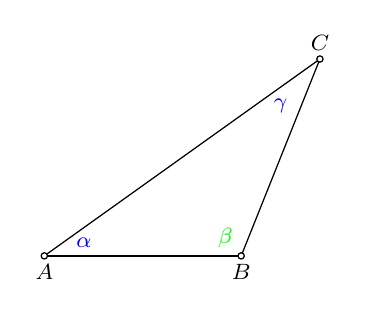
\begin{tikzpicture}
                        % \clip (0,0) rectangle (14.000000,10.000000);
                        {\footnotesize
                        
                        % Marking point A by circle
                        \draw [line width=0.016cm] (1.500000,1.500000) circle (0.040000);%
                        \draw (1.500000,1.500000) node [anchor=north] { $A$ };%
                        
                        % Marking point B by circle
                        \draw [line width=0.016cm] (4.000000,1.500000) circle (0.040000);%
                        \draw (4.000000,1.500000) node [anchor=north] { $B$ };%
                        
                        % Marking point C by circle
                        \draw [line width=0.016cm] (5.000000,4.000000) circle (0.040000);%
                        \draw (5.000000,4.000000) node [anchor=south] { $C$ };%
                        
                        % Drawing segment A B
                        \draw [line width=0.016cm] (1.540000,1.500000) -- (3.960000,1.500000);%
                        
                        % Drawing segment A C
                        \draw [line width=0.016cm] (1.532549,1.523250) -- (4.967451,3.976750);%
                        
                        % Drawing segment B C
                        \draw [line width=0.016cm] (4.014856,1.537139) -- (4.985144,3.962861);%
                        
                        % Changing color 0 0 255
                        \definecolor{r0g0b255}{rgb}{0.000000,0.000000,1.000000}%
                        \color{r0g0b255}% 
                        
                        % Marking point \gamma
                        \draw (4.500000,3.600000) node [anchor=north] { $\gamma$ };%
                        
                        % Marking point \alpha
                        \draw (1.800000,1.500000) node [anchor=south west] { $\alpha$ };%
                        
                        % Changing color 0 255 0
                        \definecolor{r0g255b0}{rgb}{0.000000,1.000000,0.000000}%
                        \color{r0g255b0}% 
                        
                        % Marking point \beta
                        \draw (4.000000,1.500000) node [anchor=south east] { $\beta$ };%
                        \color{black}
                        }
                    \end{tikzpicture}
                        
                \end{figure}

                ima en topi notranji kot, ostala dva kota ostra
                


                PRAVOKOTNI TRIKOTNIK 

                \begin{figure}[H]
                    \centering
                    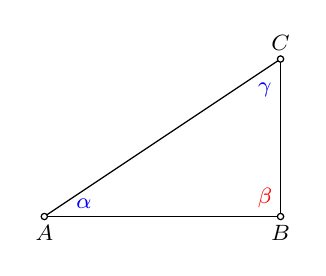
\begin{tikzpicture}
                        % \clip (0,0) rectangle (14.000000,10.000000);
                        {\footnotesize
                        
                        % Marking point A by circle
                        \draw [line width=0.016cm] (1.500000,1.500000) circle (0.040000);%
                        \draw (1.500000,1.500000) node [anchor=north] { $A$ };%
                        
                        % Marking point B by circle
                        \draw [line width=0.016cm] (4.500000,1.500000) circle (0.040000);%
                        \draw (4.500000,1.500000) node [anchor=north] { $B$ };%
                        
                        % Marking point C by circle
                        \draw [line width=0.016cm] (4.500000,3.500000) circle (0.040000);%
                        \draw (4.500000,3.500000) node [anchor=south] { $C$ };%
                        
                        % Drawing segment A B
                        \draw [line width=0.016cm] (1.540000,1.500000) -- (4.460000,1.500000);%
                        
                        % Drawing segment A C
                        \draw [line width=0.016cm] (1.533282,1.522188) -- (4.466718,3.477812);%
                        
                        % Drawing segment B C
                        \draw [line width=0.016cm] (4.500000,1.540000) -- (4.500000,3.460000);%
                        
                        % Changing color 0 0 255
                        \definecolor{r0g0b255}{rgb}{0.000000,0.000000,1.000000}%
                        \color{r0g0b255}% 
                        
                        % Marking point \gamma
                        \draw (4.300000,3.300000) node [anchor=north] { $\gamma$ };%
                        
                        % Marking point \alpha
                        \draw (1.800000,1.500000) node [anchor=south west] { $\alpha$ };%
                        
                        % Changing color 255 0 0
                        \definecolor{r255g0b0}{rgb}{1.000000,0.000000,0.000000}%
                        \color{r255g0b0}% 
                        
                        % Marking point \beta
                        \draw (4.500000,1.500000) node [anchor=south east] { $\beta$ };%
                        \color{black}
                        }
                    \end{tikzpicture}
                        
                \end{figure}

                ima en pravi notranji kot, ostala dva kot ostra
                


